\documentclass{article}

\usepackage{times}
\usepackage{amssymb, amsmath, amsthm}
\usepackage[margin=1.375in]{geometry}
\usepackage{enumitem}
\usepackage{graphicx}
\usepackage{float}
\usepackage{tikz}
\usetikzlibrary{calc}

\newenvironment{axioms}
 {\enumerate[label=\textbf{A\arabic*.}, ref=A\arabic*]}
 {\endenumerate}
\makeatletter
\newcommand\varitem[1]{\item[\textbf{A\arabic{enumi}\rlap{$#1$}.}]%
  \edef\@currentlabel{A\arabic{enumi}{$#1$}}}
\makeatother

\newtheorem{theorem}{Theorem}[section]
\newtheorem{corollary}{Corollary}[theorem]
\newtheorem{lemma}[theorem]{Lemma}

\begin{document}

\title{Projective Incidence Geometries and Models}
\author{Philip Warton}
\date{\today}
\maketitle
\tableofcontents
\newpage
\section{Introduction}

When talking about geometry, there are many rules, theorems, and axioms that one takes for granted. One could therefore assume that geometry as a whole is quite complex. In this sense, finite geometries are the minimalist geometries, where the rules are as simple as possible. This paper looks to explore the finite geometries, and find the more complicated analogues of finite projective geometries such as Fano's projective plane. First, we will introduce finite geometries that we know and understand already,  to give a basis for understanding, and then go beyond this. \\\\
To go further requires that we have a firm understanding of what is unique about Fano's plane and what axioms should be kept or altered when attempting to find patterns in these higher geometries. Though searching for patterns may be interesting, what is most insightful is to show exactly why a certain geometry functions the way it does. For this reason we will make claims about the finite projective planes and provide proofs for these claims, in the hopes that the process of showing why a geometry is a certain way will bring to light what patterns lie underneath.
\subsection{Incidence Geometry}
It is important that we first answer the question: what is an incidence geometry? What does it mean for a geometry to be finite? In typical two-dimensional Euclidean geometry, we have two coordinates, $x$ and $y$, that determine a point. Our only restriction is that $x$ and $y$ must be real numbers (in modern interpretations of Euclidean geometry). Since there are infinitely many real numbers, by extension there are infinitely many Euclidean points. Since any two points determine a single line --- the straight line passing through both --- there are infinitely many lines as well. \\

So how would one construct a finite geometry? One might attempt to look at the Euclidean plane where points are restricted to the Cartesian product of the interval $[0,1]$ with itself, that is, $([0,1] \times [0,1])$. While we have certainly made a smaller geometry, it is certainly not finite as $[0,1]$ is a compact set with infinitely many distinct numbers. So let us take only lattice points from this geometry in order to avoid the infinitesimals, as in let $x,y \in \mathbb{Z}$. This leaves us with four points $A = (0,0), B = (0,1), C = (1,0)$, and $D=(1,1)$. Now we have a proper finite geometry. Let us ignore notions of distance and angle, and focus solely on the incidence properties of this geometry: points, lines and their intersections. \\ 

Assume that the familiar Euclidean property that 2 points determine a line still holds. Then, we know that there is a line through $(0,0)$ and $(0,1)$, another through $(0,0)$ and $(1,0)$, and so on for each combination of points. Each line is drawn out in \fbox{Figure 1}.

\begin{figure}[h]
\centering
  \includegraphics[scale=.3]{final_paper_plot_1}
  \caption{Finite Euclidean Geometry}
  \label{fig:boat1}
\end{figure}

The interesting results occure when we ask questions such as: Do $\overline{AD}$ and $\overline{BC}$ intersect? They certainly appear to intersect. However, we say that two lines if they meet at a point, i.e. if they share a point of intersection. By this definition, no such point exists, because we have not defined that point $(0.5,0.5)$ in our geometry. We say that two lines are parallel if they do not intersect, and by this definition the two crossing lines are parallel. This examination of exclusively the points and lines is at the core of finite geometries, and in fact, what we have described here is a model for the four point affine plane geometry [1].

\subsection{Desired Results}
We wish to find an incidence geometry where there are no parallel lines. This quickly becomes difficult to model using the Euclidean plane and Euclidean lines. We begin to bend and stretch our lines to make the models fit the geometries they represent. While these ideas may seem bizzare, the underlying geometries are strong enough to extend to even more advanced structures, such as the real and complex projective planes. The intent of this paper, however, is to increase the complexity of the projective plane while remaining in the world of finite geometries. 

\section{Projective Planes}
Projective geometries are built upon a lack of parallelism. A crucial characteristic of projective geometry is that all lines intersect somewhere. The implications of this property are far and wide, especially so in the real and complex projective planes. However, in finite geometries, this means that we are limited to a much smaller number of geometries. One of the only geometric notions that we have so far is that two points must determine only one line. But let us add the projective property, and see what geometries are still available to us. \\

The simplest geometry here would be one point which lies on one line. To eliminate this case let us make a small adjustment and say that not all points will be co-linear. Then, we move to the three point projective plane, as seen in \fbox{Figure 2}. 

\begin{figure}[h]
\caption{The Three Point Projective Plane}
\begin{center}
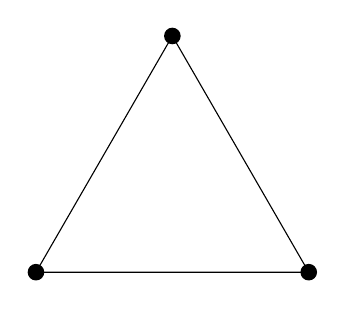
\begin{tikzpicture}
  \draw \foreach \a in {30,150,270}{}
        (90:2)  -- (210:2) -- (330:2) -- cycle;
  \fill \foreach \p in {(90:2),(210:2),(330:2)}
        {\p circle(3pt)};
\end{tikzpicture}
\end{center}
\end{figure}

It is clear that there are no parallel lines, and one more thing to note is that there are exactly as many points as there are lines. Projective geometries are also characterized by this duality of points and lines, in that the two notions are interchangable. Proofs and ideas that can be shown using points can similarly be shown using lines, and vice versa. If we attempt to make such a geometry using only four points, we end up with the four point affine plane that we introduced earlier. This geometry certainly has parallel lines, and any attempt to remedy this results in a violation of the rule that states 2 points determine exactly one line. Which leads us to the first interesting projective plane.

\section{Fano Plane}

This geometry inherets the rules we have discussed prior, and one more key property. Every line has exactly 3 points. The rules, or more formally, axioms, are the following [1].
\begin{axioms}
  \item There exists at least one line.
  \item Every line has exactly three points.
  \item Not all points are on one line.
  \item Two points determine a single line.
  \item For every pair of lines, there exists a point that is on both.
\end{axioms}
This geometry can be modeled as in \fbox{Figure 3}.

\begin{figure}[h]
\begin{center}
\caption{The Fano Plane}
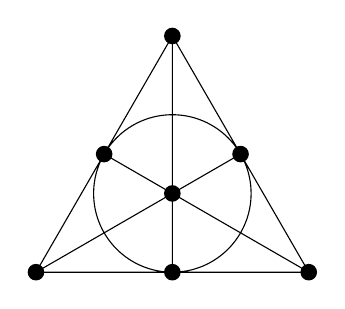
\begin{tikzpicture}
  \draw \foreach \a in {30,150,270}{(\a:1)  -- (180+\a:2)}
        (90:2)  -- (210:2) -- (330:2) -- cycle
        (0:0) circle (1);
  \fill \foreach \p in {(0:0),(30:1),(90:2),(150:1),(210:2),(270:1),(330:2)}
        {\p circle(3pt)};
\end{tikzpicture}
\end{center}
\end{figure}

One thing that may appear odd is that there is a circle, when finite geometries are restricted only to points and lines. This happens to be an obstacle that one must overcome when dealing with such geometries. It is not always the case that straight Euclidean lines can model a different geometry, so one must look at the circle inscribed in the triangle and consider it a line. There are some interesting results that come about in finding this geometry. \\

The first is that there are exactly 7 points and 7 lines. This is once again caused by the dual nature of projective geometries, and the number of points and lines depends greatly on \fbox{$\mathbf{A2}$}. Since the axiom states that every line has 3 points that lie on it, we call this geometry the order 3 projective plane. The next result is that every pair of lines has exactly one point of intersection. There are no lines that are parallel to each other, nor are there any pairs of lines that intersect at more than one point. One final interesting property to note is that every point is on exactly three lines. This is something that we can attribute to the duality of the geometry, but it is also something that can be proven from the ground up. While this geometry is fascinating in its own right, we wish to see when we go beyond 3.
\section{The Order 4 Projective Plane}
\subsubsection{Axioms}
The axioms for the order four projective plane are as follows.
\begin{axioms}
  \item There exists at least one line.
  \item Every line has exactly four points.
  \item Not all points are on one line.
  \item Two points determine a single line.
  \item For every pair of lines, there exists a point that is on both.
\end{axioms}

The first theorem for us to prove is taken directly from what we know about the Fano Plane. The proof is identical as we only changed $\mathbf{A2}$, which this theorem is independent of.

\begin{theorem}
For every pair of lines there is exactly one point of intersection.
\end{theorem}

\begin{proof}
Suppose we have a pair of lines, $l_1, l_2$. By $\mathbf{A5}$, we have one point $p$ of intersection. By contradiction, suppose there was another distinct point $q$ that was on both $l_1$ and $l_2$. Then, the two points $p$ and $q$ determine $l_1$, and also $l_2$, which violates $\mathbf{A4}$.
\end{proof}

Our next result does not come quite as easily. In fact, developing this theorem requires that we construct and keep track of many points, lines and their intersection points. Although in Fano's plane, the analogous proof was readable in written paragraph form, I intend to introduce some new notation to our incidence geometries so that we can more easily understand the geometries we construct. \\

In previous proofs, it has been enough to simply state that points $p$ and $q$ lie on some line $l$, and to say that lines $l$ and $m$ intersect at some point $p$. However, it quickly becomes obvious that this can become quite convoluted as the number of points and lines increase. One must read through an entire paragraph in order to recall if a point $p$ lies on a particular line $l$. \\

It is for this reason that I intend to use a table of binary values where each column represents a point, and each row represents a line. Then to check if point $p$ lies on line $l$, refer to row $l$ column $p$ and verify that a 1 is written there [2]. We can look at the four point affine plane in this way, \fbox{Figure 4}.
\begin{figure}[h]
\caption{Incidence Matrix for the Four Point Affine Plane}
\begin{center}
\begin{tabular}{ c|c|c|c|c } 
 
  & $p_1$ & $p_2$ & $p_3$ &$p_4$\\ 
\hline
 $l_1$ & 1 & 1 & 0 & 0\\
 \hline
 $l_2$ & 1 & 0 & 1 & 0\\
 \hline
 $l_3$ & 1 & 0 & 0 & 1\\
 \hline
 $l_4$ & 0 & 1 & 1 & 0\\
  \hline
 $l_5$ & 0 & 1 & 0 & 1\\
 \hline
 $l_6$ & 0 & 0 & 1 & 1\\
\end{tabular}
\end{center}
\end{figure}

Though it may not be immediately obvious, this model will be useful for checking certain conditions. As you may remember, when drawing the four point affine plane, there were two lines that appeared to cross but did not intersect. With this model, no such comprimise must be made. Should you look at two lines $l_3$ and $l_4$, it is clear if they share a point or not, as seen in \fbox{Figure 5}.
\begin{figure}[h]
\caption{Checking for Intersection}
\begin{center}
\begin{tabular}{ c|c|c|c|c } 
 
  & $p_1$ & $p_2$ & $p_3$ &$p_4$\\ 
 \hline
 $l_3$ & 1 & 0 & 0 & 1\\
 \hline
 $l_4$ & 0 & 1 & 1 & 0\\
\end{tabular}
\end{center}
\end{figure}
 In this case $l_3$ and $l_4$ are parallel. \\
 
 With this in mind, we introduce the next, and seemingly most important, theorem.
 \begin{theorem}
 There are exactly 13 points and 13 lines.
 \end{theorem}
 
 \begin{proof}
 By $\mathbf{A1}$, there exists a line $l_1$, and by $\mathbf{A2}$, there are exactly four points on this line, which we will call $p_1, p_2, p_3, p_4$. Because of $\mathbf{A5}$, there must exist an additional point $p_5$ that is not on $l_1$. Then, $p_5$ and $p_1$ must determine a new line $l_2$. Otherwise, $p_5$ would lie on $l_1$ and $\mathbf{A2}$ would be violated. 
 \begin{figure}[h]
 \caption{Existence of 5 Points}
 \begin{center}
\begin{tabular}{ c|c|c|c|c|c } 
 
  & $p_1$ & $p_2$ & $p_3$ &$p_4$ &$p_5$\\ 
 \hline
 $l_1$ & 1 & 1 & 1 & 1 & 0\\
 \hline
 $l_2$ & 1 & 0 & 0 & 0& 1\\
\end{tabular}
\end{center}
\end{figure}
We must construct additional points $p_6, p_7$ that lie on $l_2$, so that $l_2$ has four points on it. If we choose any of our previous points, then $l_1$ and $l_2$ would have more than one point of intersection, violating \fbox{Theorem 2.1}. Similarly, there must be a line determined by $p_5$ and $p_2$ that is not $l_1$ or $l_2$, since if $p_1$ and $p_2$ both were on a line other than $l_1$, $\mathbf{A4}$ would be violated. We will call this new line $l_3$. We must construct two more points $p_8, p_9$ that lie on $l_3$. Then, $l_4$ consists of points $p_3, p_5, p_{10}, p_{11}$, and finally $l_5$ contains $p_4, p_5, p_{12}, p_{13}$. At this point, let us omit zeroes from our incidence tables for visual clarity.
\begin{figure}[h]
\caption{Existence of 13 Points}
\begin{center}
\begin{tabular}{ c|c|c|c|c|c|c|c|c|c|c|c|c|c } 
 
  & $p_1$ & $p_2$ & $p_3$ &$p_4$ &$p_5$ &$p_6$ &$p_7$ &$p_8$ &$p_9$  &$p_{10}$&$p_{11}$&$p_{12}$&$p_{13}$ \\ 
\hline
 $l_1$ & 1 & 1 & 1 & 1 &  &&& &&&&& \\ 
 \hline
 $l_2$ & 1 & &&&1&1&1&&&&&& \\
 \hline
 $l_3$ & &1&&&1&&&1&1&&&&\\
 \hline
 $l_4$ &  &  & 1 &  &1 & &&&&1&1&&\\
 \hline
 $l_5$ & &&&1&1&&&&&&&1&1\\


\end{tabular}
\end{center}
\end{figure}
We now have the existence of 13 points. We will return to the number of points --- and showing that there are only 13 --- after we have shown the existence of 13 lines. \\

So far we have shown the existence of 5 lines. What we have so far is not complete. By $\mathbf{A4}$, $p_1$ and $p_8$ must determine a single line. This must be a new line $l_6$, otherwise we would need to say that one of our current lines is incident with another point, which would cause there to be 5 points on one line, violating $\mathbf{A2}$. Similarly, another line will be determined by $p_1$ and $p_9$. Since $p_8$ and $p_9$ determine the line $l_3$, if $p_1$, $p_8$, and $p_9$ were co-linear then $p_8, p_9$ would determine $l_3$ and $l_6$, therefore there is a new line $l_7$ determined by $p_1$ and $p_9$.

\begin{figure}[h]
\caption{Showing Existence of More Lines}
\begin{center}
\begin{tabular}{ c|c|c|c|c|c|c|c|c|c|c|c|c|c } 
  & $p_1$ & $p_2$ & $p_3$ &$p_4$ &$p_5$ &$p_6$ &$p_7$ &$p_8$ &$p_9$  &$p_{10}$&$p_{11}$&$p_{12}$&$p_{13}$ \\ 
\hline
 $l_1$ & 1 & 1 & 1 & 1 &  &&& &&&&& \\ 
 \hline
 $l_2$ & 1 & &&&1&1&1&&&&&& \\
 \hline
 $l_3$ & &1&&&1&&&1&1&&&&\\
 \hline
 $l_4$ &  &  & 1 &  &1 & &&&&1&1&&\\
 \hline
 $l_5$ & &&&1&1&&&&&&&1&1\\
 \hline
 $l_6$ &1&&&&&&&1&?&?&?&?&? \\
 \hline
 $l_7$ &1&&&&&&&&1&?&?&?&?\\
 \end{tabular}
 \end{center}
 \end{figure}
Since two points must determine a line, we say that $p_2$ and $p_6$ must determine some line. If we try to do this on some existing line, we violate $\mathbf{A2}$, so we must construct an eigth line $l_8$ which is incident with $p_2$ and $p_6$. Similarly, a line must be determined by $p_2$ and $p_7$. If we choose $l_1, l_2, \dots l_5$, we violate $\mathbf{A2}$. If we choose $l_6, \dots, l_8$, we violate $\mathbf{A4}$. Therefore we introduce a ninth line $l_9$ on which both $p_2$, and $p_7$ lie. \\

Simliarly, we say that the pairs $(p_3,p_6), (p_3,p_7), (p_4, p_6), (p_4,p_7)$ must all introduce new lines $l_{10} - l_{13}$. The prior argument that having these pairs points determine $l_1, \dots, l_5$ will mean a line will have more than four points still holds. So too does the argument that having the points determine any other previous line will mean two points determine more than one line. Therefore we know that there exists 13 lines as depicted in \fbox{Figure 9}.

\begin{figure}[h]
\caption{Showing Existence of 13 Lines}
\begin{center}
\begin{tabular}{ c|c|c|c|c|c|c|c|c|c|c|c|c|c } 
 
  & $p_1$ & $p_2$ & $p_3$ &$p_4$ &$p_5$ &$p_6$ &$p_7$ &$p_8$ &$p_9$  &$p_{10}$&$p_{11}$&$p_{12}$&$p_{13}$ \\ 
\hline
 $l_1$ & 1 & 1 & 1 & 1 &  &&& &&&&& \\ 
 \hline
 $l_2$ & 1 & &&&1&1&1&&&&&& \\
 \hline
 $l_3$ & &1&&&1&&&1&1&&&&\\
 \hline
 $l_4$ &  &  & 1 &  &1 & &&&&1&1&&\\
 \hline
 $l_5$ & &&&1&1&&&&&&&1&1\\
 \hline
 $l_6$ &1&&&&&&&1&?&?&?&?&? \\
 \hline
 $l_7$ &1&&&&&&&&1&?&?&?&?\\
 \hline
 $l_8$ &&1&&&&1&?&?&?&?&?&?&?\\
 \hline
 $l_9$ &&1&&&&&1&?&?&?&?&?&?\\
 \hline
 $l_{10}$ &&&1&&&1&?&?&?&?&?&?&?\\
 \hline
 $l_{11}$ &&&1&&&&1&?&?&?&?&?&?\\
 \hline
 $l_{12}$&&&&1&&1&?&?&?&?&?&?&?\\
 \hline
 $l_{13}$ &&&&1&&&1&?&?&?&?&?&? 

\end{tabular}
\end{center}
\end{figure}

Assume that there exists some configuration of 13 points and 13 lines that does not violate any axioms. We want to show that there can be no more than 13 points and 13 lines. Suppose there is a 14\textsuperscript{th} point $p_{14}$. Since all lines already have exactly four points, $p_{14}$ would have to be on some line $l_{14}$. This line must intersect all other lines by $\mathbf{A5}$. However, since all pairs of points in $\{p_1,p_2, \dots , p_{13}\}$ already determine one line, there is guarenteed to be a violation of axiom $\mathbf{A4}$. \\

Now suppose that there is a 14\textsuperscript{th} line. Since all lines intersect, we know that $l_{14}$ must intersect each other line at exactly one point. If we used existing points to make each line intersect, there is, again, guarenteed to be a violation of axiom $\mathbf{A4}$, as each pair of points already determine exactly one line. If we introduce a new point for any one of our points of intersection, then we violate $\mathbf{A2}$, and there is a line with five points.\\

Therefore, there are exactly 13 points and 13 lines in this geometry.
 \end{proof}
 
 One odd part of this proof was where we assume that a valid configuration of 13 points and 13 lines exist. Using trial-and-error methods the following configuration can be found as seen in \fbox{Figure 10}.
\begin{figure}[h]
\caption{Valid 13 Point Projective Geometry Configuration}
\begin{center}
\begin{tabular}{ c|c|c|c|c|c|c|c|c|c|c|c|c|c } 
 
  & $p_1$ & $p_2$ & $p_3$ &$p_4$ &$p_5$ &$p_6$ &$p_7$ &$p_8$ &$p_9$  &$p_{10}$&$p_{11}$&$p_{12}$&$p_{13}$ \\ 
\hline
 $l_1$ & 1 & 1 & 1 & 1 &  &&& &&&&& \\ 
 \hline
 $l_2$ & 1 & &&&1&1&1&&&&&& \\
 \hline
 $l_3$ & &1&&&1&&&1&1&&&&\\
 \hline
 $l_4$ &  &  & 1 &  &1 & &&&&1&1&&\\
 \hline
 $l_5$ & &&&1&1&&&&&&&1&1\\
 \hline
 $l_6$ &1&&&&&&&1&&1&&1& \\
 \hline
 $l_7$ &1&&&&&&&&1&&1&&1\\
 \hline
 $l_8$ &&1&&&&1&&&&1&&&1\\
 \hline
 $l_9$ &&1&&&&&1&&&&1&1&\\
 \hline
 $l_{10}$ &&&1&&&1&&&1&&&1&\\
 \hline
 $l_{11}$ &&&1&&&&1&1&&&&&1\\
 \hline
 $l_{12}$&&&&1&&1&&1&&&1&&\\
 \hline
 $l_{13}$ &&&&1&&&1&&1&1&&& 

\end{tabular}
\end{center}
\end{figure}


\section{The Generalized Finite Projective Plane}
Let us explore the more general version of this. Take the following axioms:

\begin{axioms}
  \item There exists at least one line.
  \item There exists $n \in \mathbb{N}$ such that every line has exactly $n$ points.
  \item Not all points are on one line.
  \item Two points determine a single line.
  \item For every pair of lines, there exists a point that is on both.
\end{axioms}

Notice how the only axiom that has changed is the second one, so that we no longer have 4 points on a line, but $n$ points. For the analogue of theorem \fbox{4.1}, it and its proof are identical as the axioms they rely on have not changed. The second theorem that states there are exactly 13 points and 13 lines must be modified. The generalized version of this theorem depends on $n$.

\begin{theorem}
If $n$ points lie on every line, then there are $n^2 - n + 1$ lines and  $n^2 - n + 1$ points.
\end{theorem}

This holds for the first few cases, for Fano's geometry, and for our 13-point projective plane. The approach to proving this theorem involves carefully counting the pairs of points that generate new lines. For example, in the proof for the 13-point projective plane, we saw that a fifth point was required so that Axiom 3 was satisfied, and that with the addition of this fifth point it must determine a line with each previous point, generating a total of five lines. Then, we saw that each of these lines must have exactly 4 points that lie on it, and this showed the existence of 13 points. There are the initial 4 points, and then the fifth point forces the construction of 4 new lines, each with 2 new points. Then we say this geometry has $4 + 1 + 4(2) = 13$ points. Similarly, if we set $n=5$ we say that by the third axiom there must exist a sixth point, besides the 5 initial co-linear points, and each pair will create a new line which will need to have 5 points that lie upon it. This creates 5 new lines with 3 new points on each which gives us $5 + 1 + 5(3) = 21$ points. We can generalize this by saying that 
\[n + 1 + n(n-2) = n^2 - n +1. \] Therefore this many points exist in the n$^{\text{th}}$ projective plane. Due to the dual nature of projective geometry, a similar proof should provide $n^2-n+1$ lines. To show there are no more points and lines follows similarly to how we proved this for the 13-point projective plane.

\section{Conclusion}
Though we quite thoroughly understand the 13-point projective plane at this point, there is a lot more to finite and projective geometries than what has been discussed so far. Subjects for further exploration include connections from the incidence geometries to combinatorics and algebra --- especially the projective planes--- and also furnished proofs for the generalized case. One more topic to look into may be the affine planes and what patterns emerge out of those geometries, or even what happens when altering different combinations of axioms. Wether it is introducing the concept of incidence or solving for elusive symmetries it is clear that the world of finite geometries has a great deal of substance to offer and is worth examination.

\begin{thebibliography}{1}

  \bibitem{notes} Edward C. Wallace and Stephen F. West {\em Roads to Geometry} 2004: Waveland Press, Inc.
 \bibitem{notes} Weisstein, Eric W. "Adjacency Matrix." From MathWorld -- A Wolfram Web Resource. http://mathworld.wolfram.com/AdjacencyMatrix.html
%https://techieme.in/graph-theory/
  \end{thebibliography}



\end{document}